
% \newpage
\section{Experiments} \label{sec:experiments}
\subsection{Posterior ratio}\label{sec:exp_ratio}

%\begin{wrapfigure}{r}{0.55\textwidth}
%    \centering
%        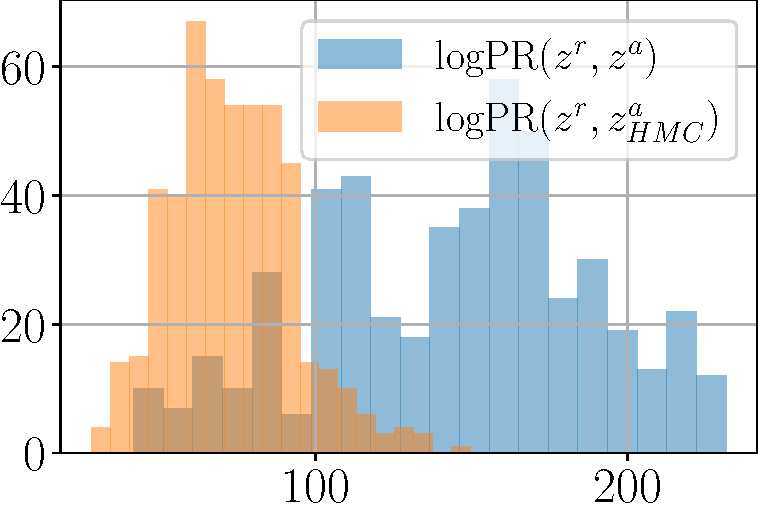
\includegraphics[width=0.45\textwidth]{pics/3_adv_att/mnist_posterior_ratio.pdf}
%    \caption{Histograms of the log posterior ratios \textcolor{blue}{before HMC (blue)} and \textcolor{orange}{after HMC (orange)} evaluated on the MNIST dataset.}
%    \label{fig:mnist_post_ratio_main}
%\end{wrapfigure}
\begin{figure}
	\centering
	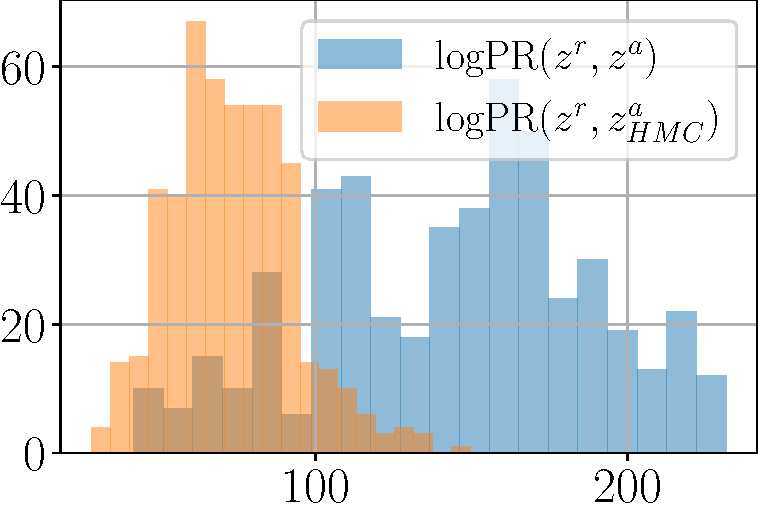
\includegraphics[width=0.5\textwidth]{pics/3_adv_att/mnist_posterior_ratio.pdf}
	\caption{Histograms of the log posterior ratios \textcolor{blue}{before HMC (blue)} and \textcolor{orange}{after HMC (orange)} evaluated on the MNIST dataset.}
	\label{fig:mnist_post_ratio_main}
\end{figure}

We motivate our method by the hypothesis that the adversarial attack "shifts" a latent code to the region of a lower posterior density, while our approach moves it back to a high posterior probability region. In Section \ref{sec:defence} we theoretically justify our hypothesis, while here we provide an additional empirical evidence.
% In order to verify our claim that applying an MCMC method allows us to counteract attacks by moving a latent code from a region of a lower posterior probability mass to a region of a higher density, we propose to quantify this effect by measuring the ratio of posteriors for $\rvz_1$ and $\rvz_2$. 
The true posterior $p(\rvz | \rvx^{r})$ is not available due to the cumbersome marginal distribution $p(\rvx^{r})$, however, we can calculate the ratio of posteriors because the marginal will cancel out. In our case, we are interested in calculating the posterior ratio between the reference and adversarial latent codes ($\rvz_1 = \rvz^r$,  $\rvz_2 = \rvz^a$) as the baseline, and the posterior ratio between the reference and adversarial code after applying the HMC ($\rvz_1 = \rvz^r$ , $\rvz_2 = \rvz^a_{\text{HMC}}$). The lower the posterior ratio, the better. For practical reasons, we use the logarithm of the posterior ratio since the logarithm does not change the monotonicity and turns products to sums:
\begin{equation}
    \log \text{PR}(\rvz_1, \rvz_2) = \log p_{\theta}(\rvx^r|\rvz_1) + \log p(\rvz_1) - \log p_{\theta}(\rvx^r| \rvz_2) - \log p(\rvz_2) .
\end{equation}
% , namely:

% \begin{align}
% \text{PR}(\rvz_1, \rvz_2) &= \tfrac{p_{\theta}(\rvz_1|\rvx^r)}{p_{\theta}(\rvz_2|\rvx^r)} \\
% &= \tfrac{p_{\theta}(\rvx^r|\rvz_1)p(\rvz_1)}{p_{\theta}(\rvx^r| \rvz_2)p(\rvz_2)} .
% \end{align}
In Figure \ref{fig:mnist_post_ratio_main} we show a plot with two histograms: one with the posterior ratio between the reference and adversarial latent codes ($\rvz_1 = \rvz^r$,  $\rvz_2 = \rvz^a$) in blue, and the second histogram of the posterior ratio between the reference and adversarial code after applying the HMC ($\rvz_1 = \rvz^r$ , $\rvz_2 = \rvz^a_{\text{HMC}}$) in orange. We observe that the histogram has moved to the left after applying the HMC. This indicates that posterior of the adversarial (in the denominator) is increasing when the HMC is used. This is precisely the effect we hoped for and this result provides an empirical evidence in favor of our hypothesis. For more details see \ref{appendix:posterior_ratio}.


% \mw{Max: corrected until here}
% In this section, we experimentally evaluate performance of the proposed approach 
% % \footnote{Our code is publicly available at \url{hidden-repository-due-to-double-blind-review}.}. 
% We perform experiments on a variety of VAE models ($\beta$-VAE, $\beta$-TCVAE and NVAE) and datasets (MNIST. Fashion MNIST, Color MNIST, CelebA).

% ==== SubSECTION ====
\subsection{VAE, $\beta$-VAE and $\beta$-TCVAE} %\texorpdfstring{
% First, we consider attacks on VAE with a single level of latent variables. 
All implementation details and hyperparameters are included in the Appendix ~\ref{appendix:experimental_details} and code repository~\footnote{\url{github.com/AKuzina/defend_vae_mcmc}}. 
\paragraph{Datasets}
VAEs are trained on the MNIST, Fashion MNIST \cite{xiao2017fashion} and Color MNIST datasets. Following \cite{Cemgil2019-vn}, we construct the Color MNIST dataset from MNIST by artificially coloring each image with seven colors (all corners of RGB cube except for black). 

% \begin{wrapfigure}{r}{0.55\textwidth}
\begin{figure}
%\vskip -5pt
    \centering
    \begin{tabular}{ccccc}
        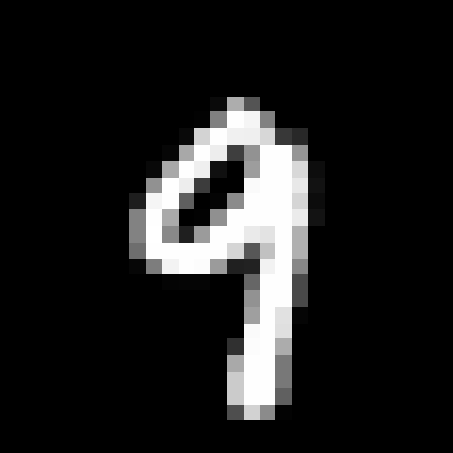
\includegraphics[width=0.1\linewidth]{pics/3_adv_att/mnist_ref_4.pdf} & 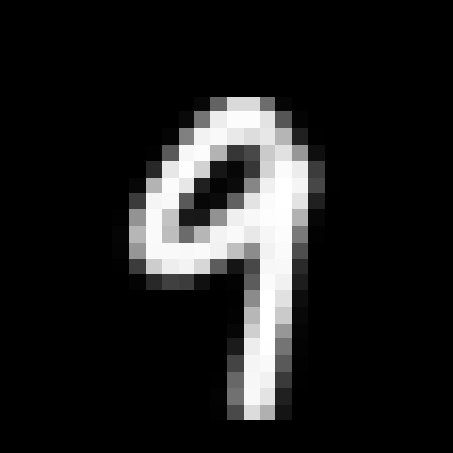
\includegraphics[width=0.1\linewidth]{pics/3_adv_att/mnist_ref_rec_4.pdf} &
        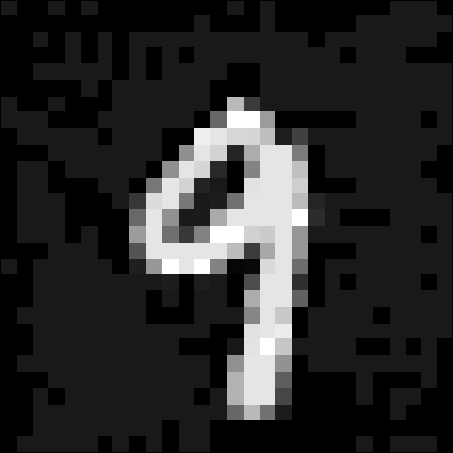
\includegraphics[width=0.1\linewidth]{pics/3_adv_att/mnist_adv_4.pdf} & 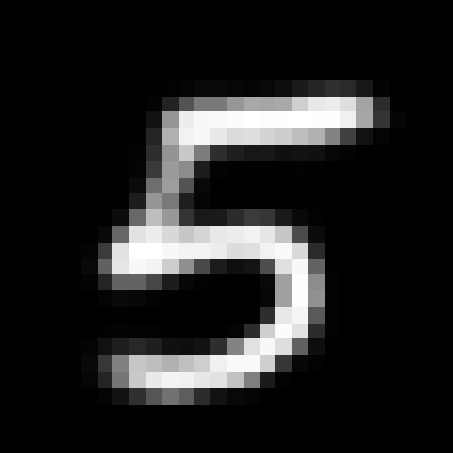
\includegraphics[width=0.1\linewidth]{pics/3_adv_att/mnist_adv_rec_4.pdf} & 
        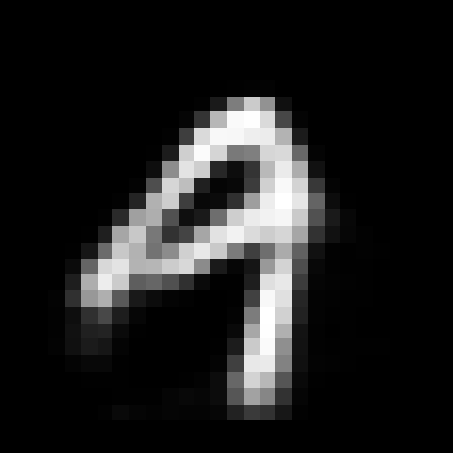
\includegraphics[width=0.1\linewidth]{pics/3_adv_att/mnist_adv_rec_hmc_4.pdf}\\
        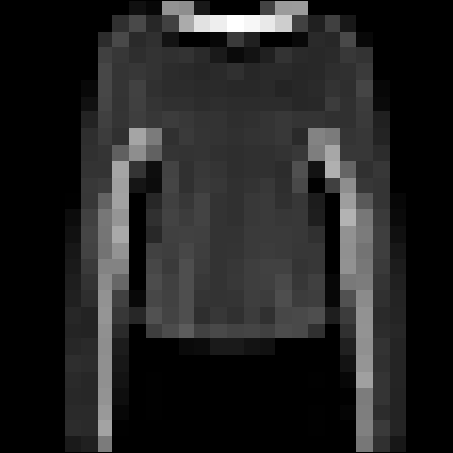
\includegraphics[width=0.1\linewidth]{pics/3_adv_att/fashion_mnist_ref_14.pdf} & 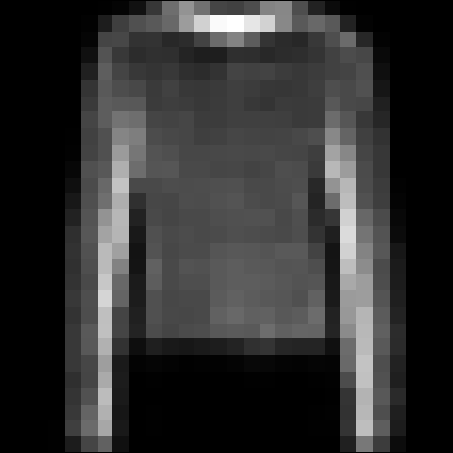
\includegraphics[width=0.1\linewidth]{pics/3_adv_att/fashion_mnist_ref_rec_14.pdf} &
        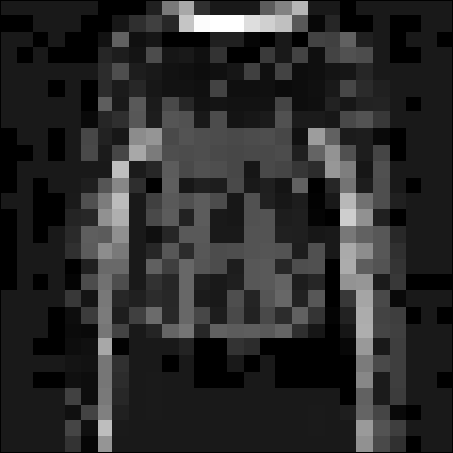
\includegraphics[width=0.1\linewidth]{pics/3_adv_att/fashion_mnist_adv_14.pdf} & 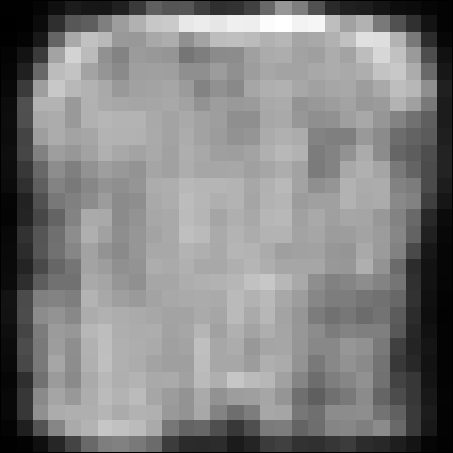
\includegraphics[width=0.1\linewidth]{pics/3_adv_att/fashion_mnist_adv_rec_14.pdf} & 
        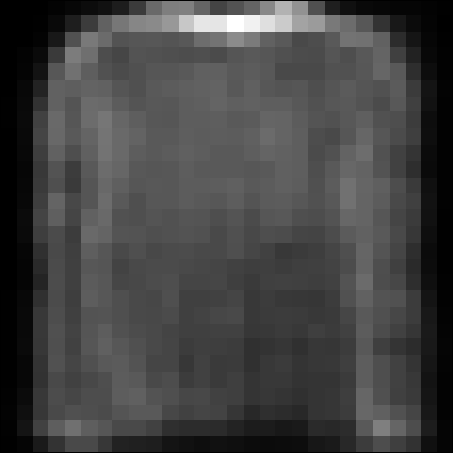
\includegraphics[width=0.1\linewidth]{pics/3_adv_att/fashion_mnist_adv_rec_hmc_14.pdf}\\
        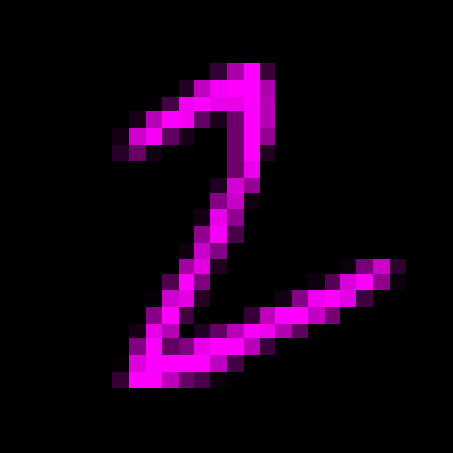
\includegraphics[width=0.1\linewidth]{pics/3_adv_att/color_mnist_ref_4.pdf} & 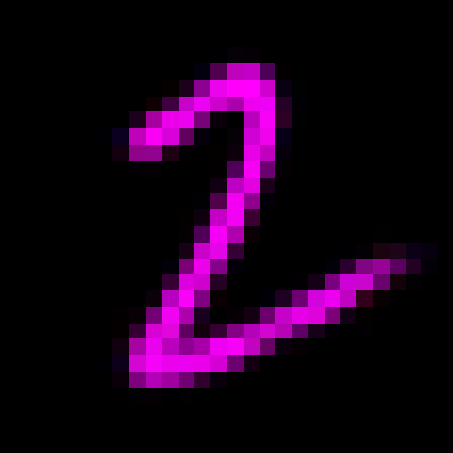
\includegraphics[width=0.1\linewidth]{pics/3_adv_att/color_mnist_ref_rec_4.pdf} &
        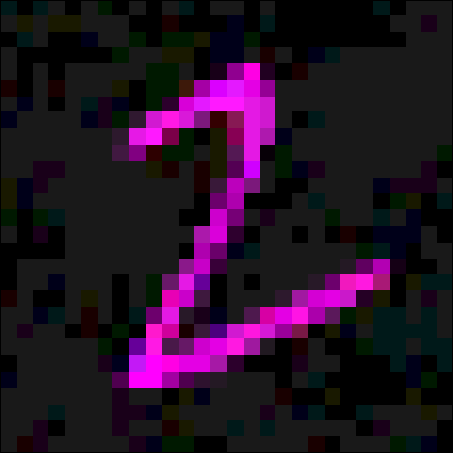
\includegraphics[width=0.1\linewidth]{pics/3_adv_att/color_mnist_adv_4.pdf} & 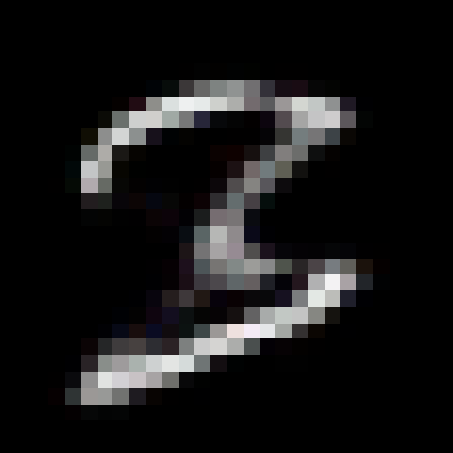
\includegraphics[width=0.1\linewidth]{pics/3_adv_att/color_mnist_adv_rec_4.pdf} & 
        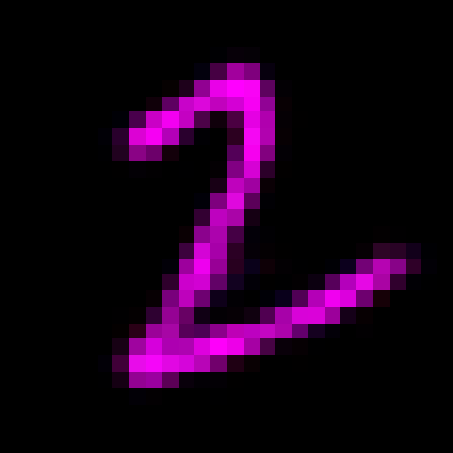
\includegraphics[width=0.1\linewidth]{pics/3_adv_att/color_mnist_adv_rec_hmc_4.pdf}\\
        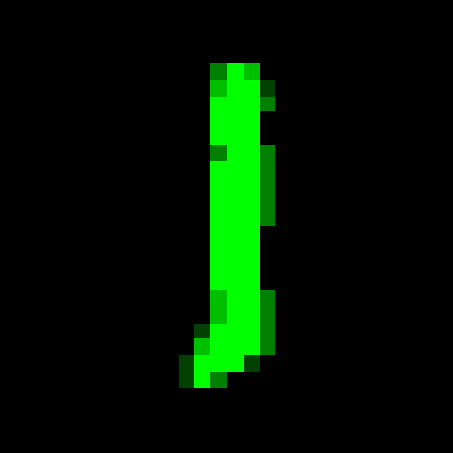
\includegraphics[width=0.1\linewidth]{pics/3_adv_att/color_mnist_ref_9.pdf} & 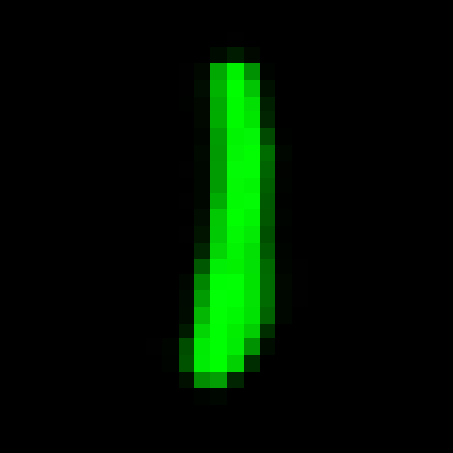
\includegraphics[width=0.1\linewidth]{pics/3_adv_att/color_mnist_ref_rec_9.pdf} &
        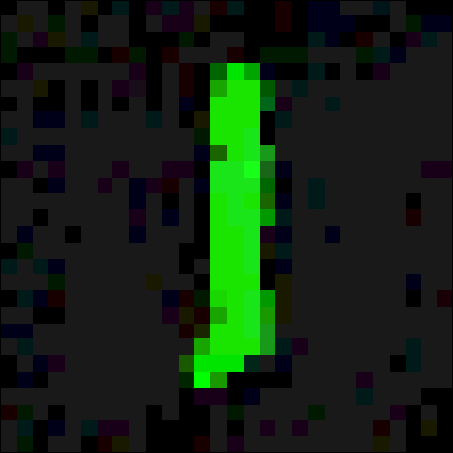
\includegraphics[width=0.1\linewidth]{pics/3_adv_att/color_mnist_adv_9.pdf} & 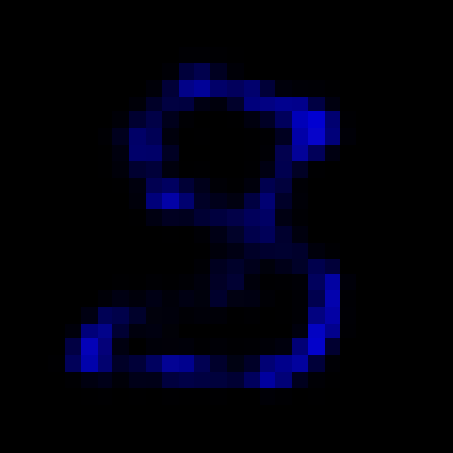
\includegraphics[width=0.1\linewidth]{pics/3_adv_att/color_mnist_adv_rec_9.pdf} & 
        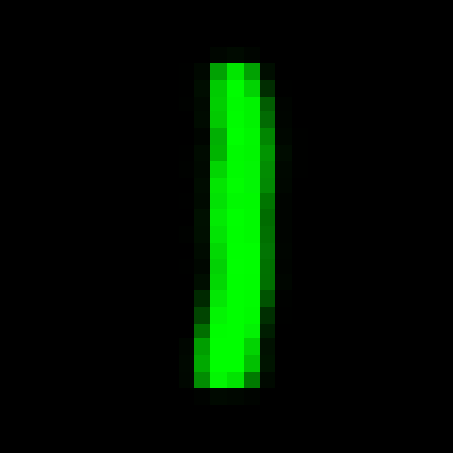
\includegraphics[width=0.1\linewidth]{pics/3_adv_att/color_mnist_adv_rec_hmc_9.pdf}\\
        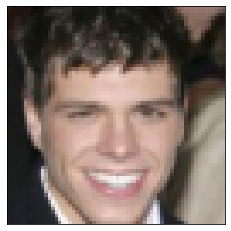
\includegraphics[width=0.1\linewidth]{pics/3_adv_att/celeba_ref_1.png} & 
\includegraphics[width=0.1\linewidth]{pics/3_adv_att/celeba_ref_rec_1.png} &
        
\includegraphics[width=0.1\linewidth]{pics/3_adv_att/celeba_adv_1.png} & 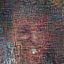
\includegraphics[width=0.1\linewidth]{pics/3_adv_att/celeba_adv_rec_1.png} & 
        
\includegraphics[width=0.1\linewidth]{pics/3_adv_att/celeba_adv_rec_hmc_1.png}\\
        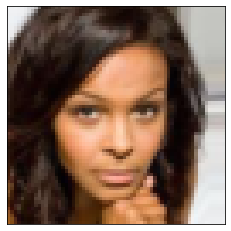
\includegraphics[width=0.1\linewidth]{pics/3_adv_att/celeba_ref_2.png} & 
\includegraphics[width=0.1\linewidth]{pics/3_adv_att/celeba_ref_rec_2.png} &
        
\includegraphics[width=0.1\linewidth]{pics/3_adv_att/celeba_adv_2.png} & 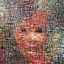
\includegraphics[width=0.1\linewidth]{pics/3_adv_att/celeba_adv_rec_2.png} & 
        
\includegraphics[width=0.1\linewidth]{pics/3_adv_att/celeba_adv_rec_hmc_2.png}\\
        (a) $\rvx^r$ & (b) $\widetilde{\rvx}^r$ & (c) $\rvx^a$ & (d) $\widetilde{\rvx}^a$ & (e) $\widetilde{\rvx}^\text{a}_{\text{HMC}}$ \\
    \end{tabular}
    \caption{Examples of (a) reference points, (b) reconstructions of the reference points, (c) adversarial points, (d) reconstructions of the adversarial points, (e) reconstructions of the adversarial points after the proposed defence (HMC). All the adversarial examples are unsupervised attacks on the encoder. Last two rows contain examples for the NVAE model discussed in Section \protect\ref{sec:nvae}}
    \label{fig:adversarial_examples}
    \vspace*{\baselineskip}
\end{figure}
% \end{wrapfigure}


\paragraph{Models}
We train vanilla fully convolutional VAEs, as well as $\beta$-VAE \cite{higgins2016beta} and $\beta$-TCVAE \cite{chen2018isolating, kim2018disentangling}. Both $\beta$-VAE and $\beta$-TCVAE modify the ELBO objective to encourage disentanglement. $\beta$-VAE weighs the KL-term in the ELBO with $\beta > 0$. It is said that the larger values of $\beta$ encourage disentangling of latent representations \cite{chen2018isolating} and improve the model robustness as observed by \cite{camuto2021towards}. $\beta$-TCVAE puts a higher weight on the total correlation (TC) term of the ELBO. Penalization of the total correlation was shown to increase the robustness of VAE adversarial attacks \cite{Willetts2019-mu}.

In Appendix \ref{appendix:beta_vae_param} we provide details of the architecture, optimization, and results on the test dataset for VAE trained with different values of $\beta$. 
We note that the optimal value in terms of the negative log-likelihood (NLL) is always $\beta=1$. Larger values of $\beta$ are supposed to improve robustness in exchange for the reconstruction quality. When evaluating the robustness of $\beta$-VAE and $\beta$-TCVAE, we train models with $\beta \in \{2, 5, 10\}$. Then, we select the value of $\beta$ that provides the most robust model in terms of the used metric. Next, we apply our defence strategy to this model to observe the potential performance improvement. 


\begin{table}[h]
\caption[][\baselineskip]{Results for unsupervised attack with radius $0.1$ and $0.2$ on MNIST and Fashion MNIST datasets. We attack the encoder (left) and the downstream classification task (right).
% Higher values correspond to more robust models.
\\\textsuperscript{$\dagger$} Our implementation.}
\vskip -0.2cm
\label{tab:mnist_attack_result}
\begin{center}
\begin{small}
\begin{sc}
\resizebox{1.0\textwidth}{!}{
\begin{tabular}{lllcc|ccc|ll}
\toprule
& & & \multicolumn{2}{c|}{$\mathrm{MSSSIM}[\widetilde{\rvx}^{r}, \widetilde{\rvx}^{a}]$ $\uparrow$} & \multicolumn{3}{c|}{Adversarial Accuracy $\uparrow$} & \multirow{2}{*}{MSE $\downarrow$}  \\
\multicolumn{3}{c}{$\|\varepsilon\|$} & 0.1 & 0.2 & 0.0 & 0.1 & 0.2           & &\\ 
\midrule
 & \multirow{3}{*}{\STAB{\rotatebox[origin=c]{90}{\small{MNIST}}}} 
 & VAE & 0.70 \tiny{(0.02)} & 0.36 \tiny{(0.03)} & \textbf{0.90} \tiny{(0.04)} & 0.08 \tiny{(0.04)} & 0.05 \tiny{(0.03)} & 578.7 \\
&& \textbf{VAE + HMC} & \textbf{0.88} \tiny{(0.01)} & \textbf{0.76} \tiny{(0.02)} & 0.76 \tiny{(0.01)} & \textbf{0.25} \tiny{(0.03)} & \textbf{0.19} \tiny{(0.03)} & \textbf{478.1} 
\\
&& $\beta$-VAE & 0.75 \tiny{(0.01)} & 0.50 \tiny{(0.03)} & 0.90 \tiny{(0.05)} & 0.11 \tiny{(0.04)} & 0.01 \tiny{(0.01)} & 824.2 \\
&& $\beta$-TCVAE\textsuperscript{$\dagger$} 
& 0.70 \tiny{(0.02)} & 0.46 \tiny{(0.03)} & 0.86 \tiny{(0.05)} & 0.05 \tiny{(0.03)} & 0.03 \tiny{(0.02)} & 828.4
\\ \midrule 
\multirow{3}{*}{\STAB{\rotatebox[origin=c]{90}{\small{Fashion}}}} &\multirow{3}{*}{\STAB{\rotatebox[origin=c]{90}{\small{MNIST}}}} 
&VAE           & 0.59 \tiny{(0.03)} & 0.47 \tiny{(0.03)} & 0.78 \tiny{(0.06)} & 0.00 \tiny{(0.01)} & 0.01 \tiny{(0.01)} & 814.2  \\
&& \textbf{VAE + HMC}    & \textbf{0.66} \tiny{(0.03)} & \textbf{0.54} \tiny{(0.03)} & 0.56 \tiny{(0.01)} & \textbf{0.14} \tiny{(0.02)} & \textbf{0.13} \tiny{(0.02)} & \textbf{764.2} \\ 
&& $\beta$-VAE & 0.52 \tiny{(0.03)} & 0.41 \tiny{(0.03)} & 0.80 \tiny{(0.05)} & 0.00 \tiny{(0.01)} & 0.00 \tiny{(0.01)} & 
1021.1\\
&& $\beta$-TCVAE\textsuperscript{$\dagger$} & 0.52 \tiny{(0.03)} & 0.42 \tiny{(0.03)} & \textbf{0.84} \tiny{(0.05)} & 0.00 \tiny{(0.01)} & 0.02 \tiny{(0.02)} & 980.4\\ 
\bottomrule
\end{tabular}
}
\end{sc}
\end{small}
\end{center}
\vspace*{\baselineskip}
\end{table}

%%%% MOVED TO APPENDIX
% \begin{figure}[t]
%     \centering
%     \begin{tabular}{ll}
%         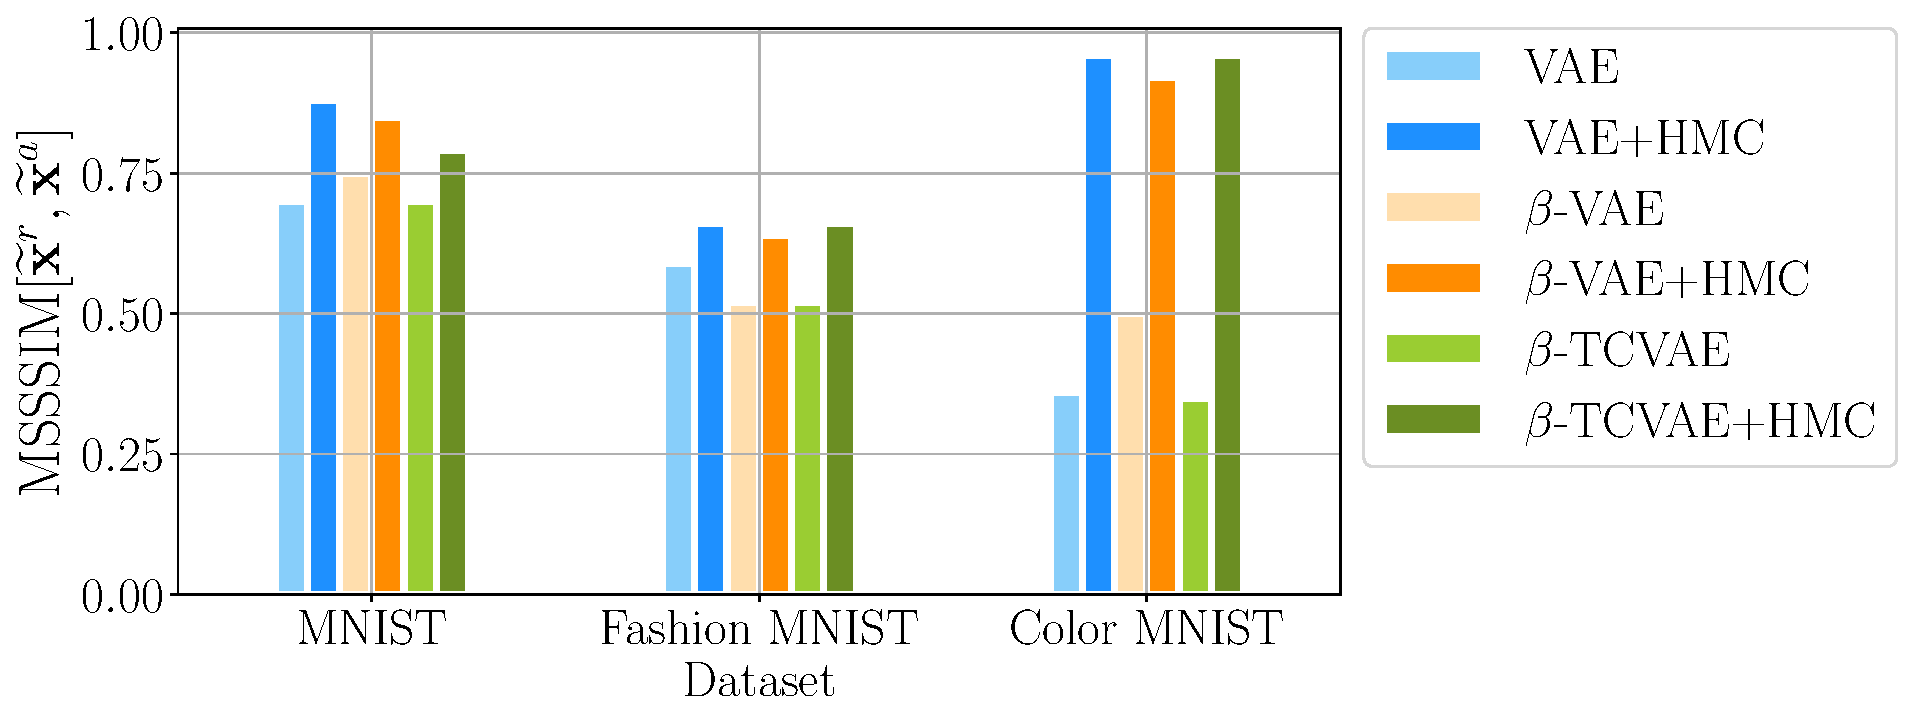
\includegraphics[width=0.5\textwidth]{img/msssim_eps_1.pdf} & 
%         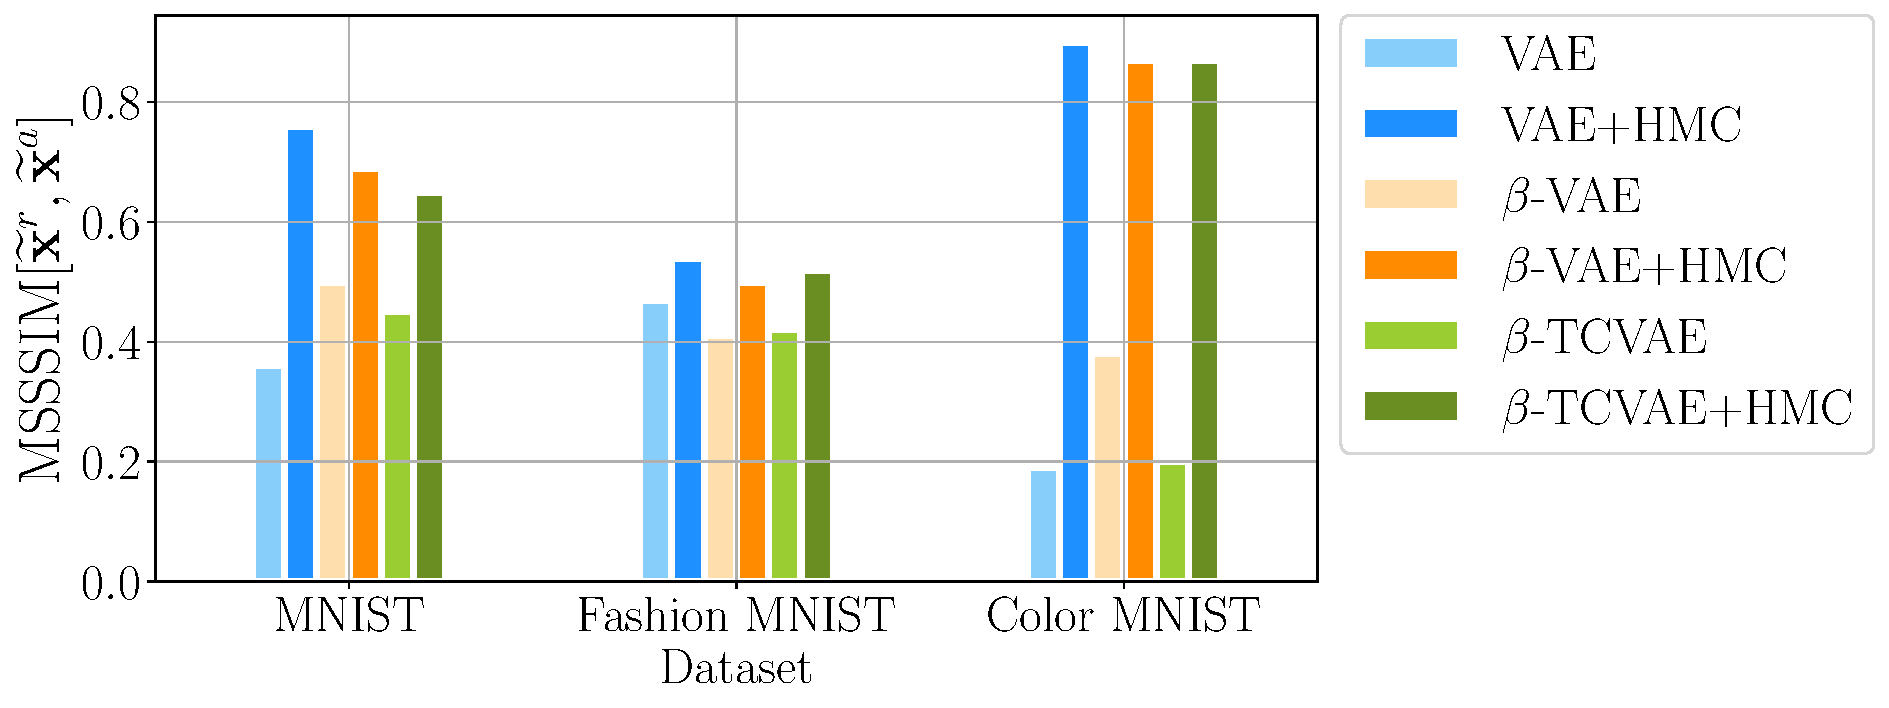
\includegraphics[width=0.5\textwidth]{img/msssim_eps_2.pdf} \\
%         \multicolumn{1}{c}{(a) $||\varepsilon ||_{\inf} = 0.1$} &
%         \multicolumn{1}{c}{(b) $||\varepsilon ||_{\inf} = 0.2$} \\
%         % (a) & (b) \\
%         % (c) & (d)
%     \end{tabular}
%     \caption{Improvement of the Reconstruction Similarity after the proposed defence. We fix the attack radius to be equal to (a) 0.1 and (b) 0.2. Higher values correspond to a more robust representations.}
%     \vskip -10pt
%     \label{fig:mnist_rec_similarity}
% \end{figure}


\begin{table}[ht]
\caption[][\baselineskip]{Results for unsupervised attack with radius $0.1$ and $0.2$ on ColorMNIST dataset. We attack the encoder (left) and the downstream classification task (right).
% Higher values correspond to more robust models.
\\ \textsuperscript{$\dagger$} Our implementation. \\
\textsuperscript{*} Values reported in \cite{cemgil2020autoencoding}, VAE implementation and evaluation protocol may differ. }
\vskip -0.2cm
\label{tab:color_mnist_attack_results}
\begin{center}
\begin{small}
\begin{sc}
\resizebox{1.03\textwidth}{!}{
\begin{tabular}{lcc|cccccc|ll}
\toprule
 & \multicolumn{2}{c|}{$\mathrm{MSSSIM}[\widetilde{\rvx}^{r}, \widetilde{\rvx}^{a}]$ $\uparrow$} & \multicolumn{6}{c|}{Adversarial Accuracy $\uparrow$} & \multirow{3}{*}{MSE$\downarrow$} &  \multirow{3}{*}{FID $\downarrow$} \\
 &     &     & \multicolumn{3}{c}{Digit} &  \multicolumn{3}{c|}{Color} & & \\
 $\|\varepsilon\|$& 0.1 & 0.2 & 0.0 & 0.1 & 0.2           & 0.0 & 0.1 & 0.2             & & \\ \midrule
% \multirow{9}{*}{\STAB{\rotatebox[origin=c]{90}{Color MNIST}}} & 
VAE & 0.36 \tiny{(0.03)} & 0.19 \tiny{(0.02)} & \textbf{1.00 \tiny{(0.00)}} & 0.04 \tiny{(0.03)} & 0.02 \tiny{(0.02)} & 1.00 \tiny{(0.00)} & 0.06 \tiny{(0.03)} & 0.06 \tiny{(0.03)} & \textbf{261} & \textbf{2.1}\\
% & 
\textbf{VAE + HMC}
& \textbf{0.96 \tiny{(0.01)}} & \textbf{0.90 \tiny{(0.01)}} & 0.42 \tiny{(0.01)} & 0.16 \tiny{(0.02)} & 0.11 \tiny{(0.02)} & 1.00 \tiny{(0.00)} & 0.68 \tiny{(0.03)} & 0.62 \tiny{(0.03)} & \textbf{206} & \textbf{2.1}\\
\midrule
$\beta$-VAE 
& 
0.75 \tiny{(0.01)} & 0.5 \tiny{(0.03)} & 0.88 \tiny{(0.04)} & 0.08 \tiny{(0.04)} & 0.05 \tiny{(0.03)} & 1.00 \tiny{(0.00)} & 0.21 \tiny{(0.06)} & 0.18 \tiny{(0.05)} & 366 & 2.4\\
$\beta$-TCVAE\textsuperscript{$\dagger$} 
& 
0.35 \tiny{(0.02)} & 0.23 \tiny{(0.02)} & 0.94 \tiny{(0.04)} & 0.08 \tiny{(0.04)} & 0.05 \tiny{(0.03)} & 1.00 \tiny{(0.00)} & 0.06 \tiny{(0.03)} & 0.05 \tiny{(0.02)} & 366 & 3.0\\
% & 
$\text{SE}_{0.1}$\textsuperscript{*}
& N/A                & N/A                & 0.94 \tiny{(N/A)}  & 0.89 \tiny{(N/A)}  & 0.02 \tiny{(N/A)}  & 1.00 \tiny{(N/A)}  & 1.00 \tiny{(N/A)}  & 0.22 \tiny{(N/A)}  & 1372 & 13.0\\
% & 
$\text{SE}_{0.2}$\textsuperscript{*}
& N/A                & N/A                & 0.95 \tiny{(N/A)}  & 0.92 \tiny{(N/A)}  & \textbf{0.87 \tiny{(N/A)}}  & 1.00 \tiny{(N/A)}  & 1.00 \tiny{(N/A)}  & \textbf{1.00 \tiny{(N/A)}}  & 1375 & 11.7 \\
% & 
AVAE\textsuperscript{*} 
& N/A                & N/A                & 0.97 \tiny{(N/A)}  & 0.88 \tiny{(N/A)}  & 0.55 \tiny{(N/A)}  & 1.00 \tiny{(N/A)}  & 1.00 \tiny{(N/A)} & 0.88 \tiny{(N/A)}  & 1372 & 15.5\\
% & 
$\text{SE}_{0.1}$-AVAE\textsuperscript{*}
& N/A                & N/A                & 0.97 \tiny{(N/A)}  & \textbf{0.94 \tiny{(N/A)}}  & 0.25 \tiny{(N/A)}  & 1.00 \tiny{(N/A)}  & 1.00 \tiny{(N/A)}  & 0.60 \tiny{(N/A)}  & 1373 & 13.9\\
% & 
$\text{SE}_{0.2}$-AVAE\textsuperscript{*} 
& N/A                & N/A                & 0.98 \tiny{(N/A)}  & \textbf{0.94 \tiny{(N/A)}}  & 0.80 \tiny{(N/A)}  & 1.00 \tiny{(N/A)}  & 1.00 \tiny{(N/A)}  & 0.83 \tiny{(N/A)}  & 1374 & 13.9\\
% & 
AVAE-SS\textsuperscript{*} 
& N/A                & N/A                & 0.94 \tiny{(N/A)}  & 0.73 \tiny{(N/A)}  & 0.21 \tiny{(N/A)}  & 1.00 \tiny{(N/A)}  & 1.00 \tiny{(N/A)}  & 0.57 \tiny{(N/A)}  & 1379 & 12.4\\
\bottomrule
\end{tabular}}
\end{sc}
\end{small}
\end{center}
\vspace*{\baselineskip}
\end{table}

%%%% MOVED TO APPENDIX
% \begin{figure}[t]
%     \centering
%     \begin{tabular}{ll}
%         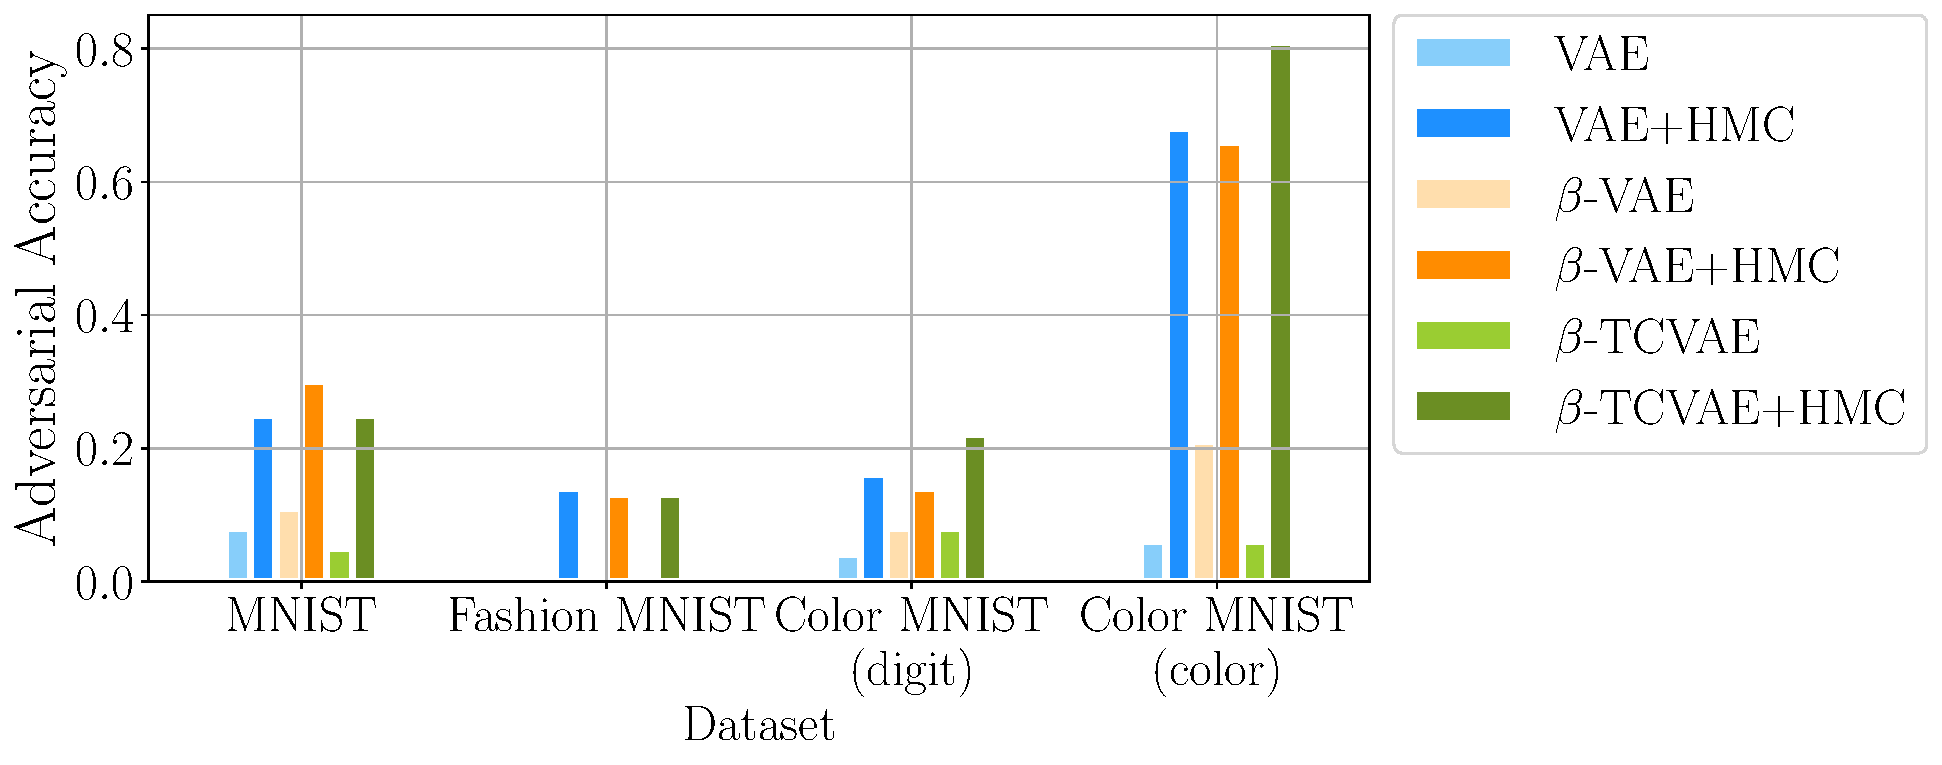
\includegraphics[width=0.5\textwidth]{img/adv_acc_eps_1.pdf} &
%         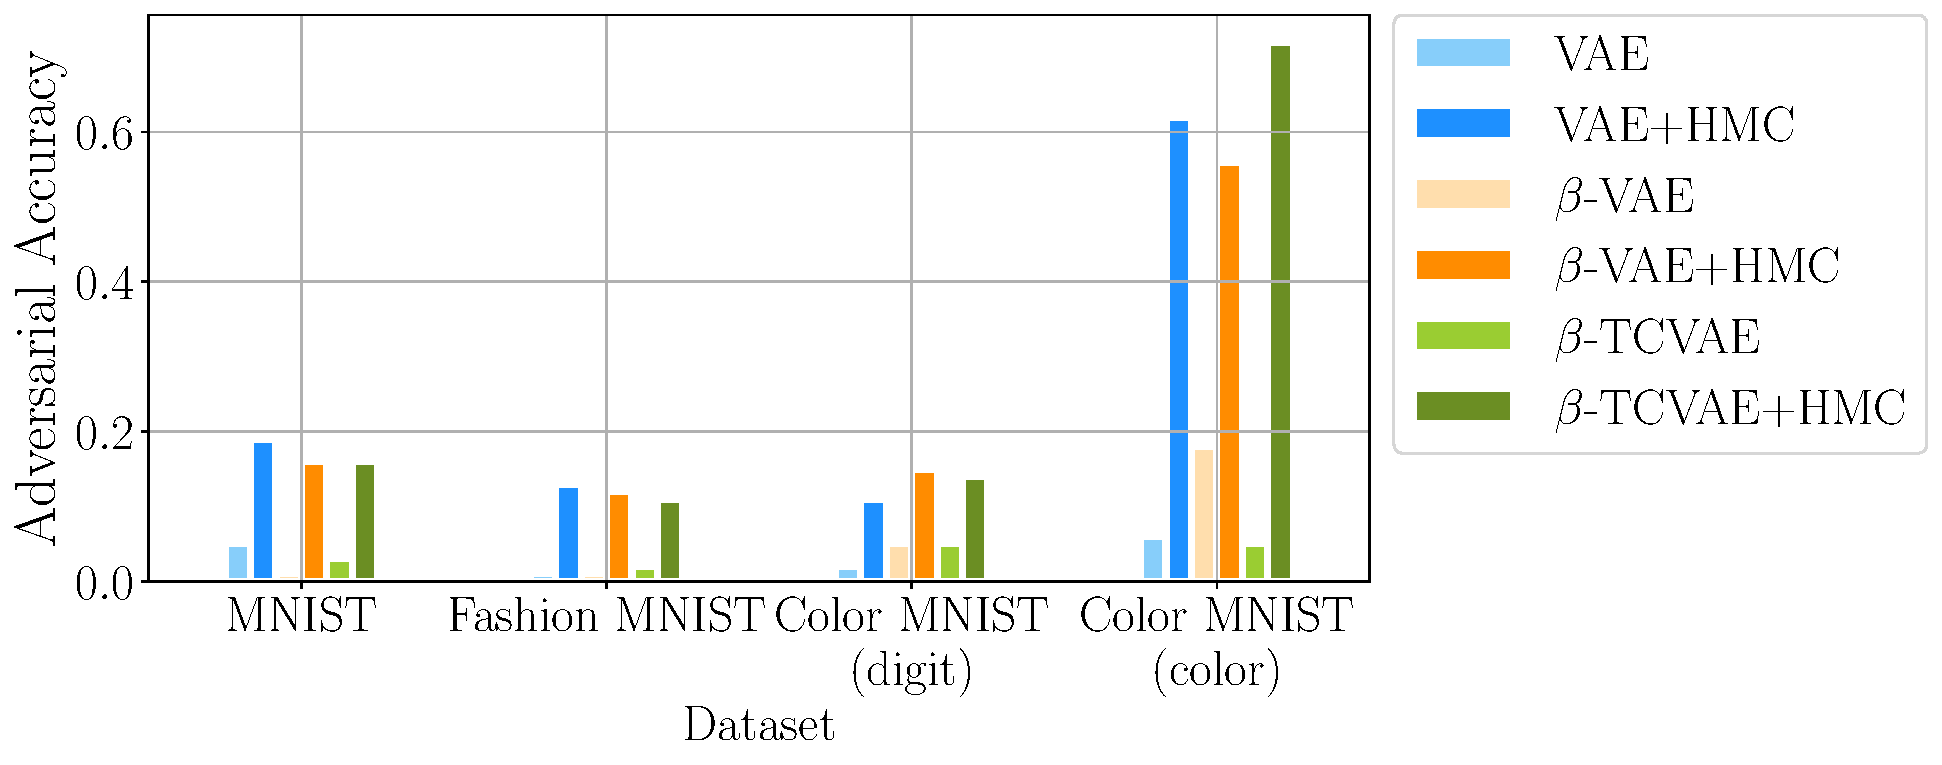
\includegraphics[width=0.5\textwidth]{img/adv_acc_eps_2.pdf} \\
%         \multicolumn{1}{c}{(a) $||\varepsilon ||_{\inf} = 0.1$} &
%         \multicolumn{1}{c}{(b) $||\varepsilon ||_{\inf} = 0.2$} \\
%         % (a) & (b) \\
%         % (c) & (d)
%     \end{tabular}
%     % \vskip -10pt
%     \caption{Improvement of the Adversarial Accuracy after proposed defence. We fix the attack radius to be equal to (a) 0.1 and (b) 0.2.}
%     \vskip -10pt
%     \label{fig:mnist_adv_acc}
% \end{figure}
\paragraph{Attacks on the Encoder} 
In the first setup, we assume that the attacker has access to the encoder of the model $\Enc{z}{x}$ {\cite{barrett2021certifiably, Gondim-Ribeiro2018-cu, Willetts2019-mu}. We use the projected gradient descent (PGD) with 50 steps to maximize the symmetric KL-divergence in the unsupervised setting (\eqref{eq:objective_unsup}). We train 10 adversarial attacks (with different random initialization) for each of 50 reference points. See Appendix \ref{appendix:vae_attack} for the details. We report similarity between the reconstruction of the adversarial and reference point as a measure of the robustness (see Section \ref{sect:adversarial_attacks}). 

\paragraph{Attacks on the downstream task} 
In this setup, we examine how the proposed approach can aleviate the effect of the attack on the downstream tasks in the latent space. For this purpose, we follow the procedure from \cite{cemgil2020autoencoding, Cemgil2019-vn}. Once the VAE is trained, we learn a linear classifier using the mean mappings as features. For the MNIST and Fashion MNIST datasets, we have the 10-class classification problem (digits in the former and pieces of clothing in the latter case). For the ColorMNIST dataset, we consider two classification tasks: the digit classification (10 classes), and the color classification (7 classes). We construct the attack to fool the classifier. See Appendix \ref{appendix:vae_attack} for the details.


\paragraph{Results} 
In Tables \ref{tab:mnist_attack_result} and \ref{tab:color_mnist_attack_results}, we compare our method (VAE + HMC) with the vanilla VAE with other methods in the literature. We report more results and the extended comparison in the Appendix \ref{appendix:beta_vae} where we show that our method combined with $\beta$-VAE and $\beta$-TCVAE leads to the increased robustness. For MNIST and Fashion MNIST (Table \ref{tab:mnist_attack_result}), we observe that the vanilla VAE with the HMC is more robust than $\beta$-VAE and $\beta$-TCVAE. The latter model was shown to be more robust to the latent space attack \cite{Willetts2019-mu}. Still, in our experiments (on different datasets), we could not observe the consistent improvement over the vanilla VAE, when using it with a single level of latent variables. 

In Table \ref{tab:color_mnist_attack_results} we report the result on the ColorMNIST dataset. Here, we additionally compare the adversarial accuracy for our method with the Smooth Encoders (SE) and Autoencoding Variational Autoencoder (AVAE) methods \cite{cemgil2020autoencoding, Cemgil2019-vn}.
% We notice that these methods provide higher adversarial accuracy. However, we have also observed a large discrepancy in terms of the MSE and FID scores of the model itself compared to our experiments, which we suspect might be a result of a mistake in \cite{cemgil2020autoencoding, Cemgil2019-vn}.
% \footnote{We have gotten in touch with the authors, who are kindly working with us to address this issue}

Lastly, we would like to highlight that our defence strategy can be also combined with all the above VAE modifications. One advantage of our approach is that it does not require changing the training procedure of a VAE and, as a result, it does not decrease the quality of the generated images. 
Moreover, we can apply the same procedure to reconstruct the non-corrupted points and it will improve the reconstruction error. 
This result can be seen in the Tables \ref{tab:mnist_attack_result} and \ref{tab:color_mnist_attack_results} and it goes in line with the results of the \cite{salimans2015markov}, where MCMC was used to improve the VAE performance. 
% SE and AVAE methods without any restrictions.  
% Another advantage of our approach is that it does not require changing the training procedure of a VAE and, as a result, it does not decrease the quality of the generated images. \ak{As we observe from the columns \textbf{MSE} and \textbf{FID}, the quality of the vanilla VAE is always better compared to the models with modified training objectives. MODIFY: Mention bridging the gap paper.} We depict several examples of the reconstructions of the attacked point in Figure \ref{fig:adversarial_examples}.


% In Figure \ref{fig:mnist_rec_similarity}, we show how similarity between the reconstructions of the reference and adversarial points increases after the proposed defence is applied. This metric consistently improves for all the datasets, radii and models considered. In Figure \ref{fig:adversarial_examples}, we plot examples for each of the datasets considered (see subsection \ref{sec:nvae} for more details on CelebA experiments). The first two columns contain reference points and their reconstructions (columns a \& b). Then we plot the adversarial input (column c) and its reconstruction without the defence (column d). Finally, we provide the reconstruction with the defence applied (column e) that is much closer to the reconstruction of the reference point.
 


% ==== SubSECTION ====
\begin{figure}[t]
    % \centering
    \begin{adjustbox}{center}
    \begin{tabular}{llll}
        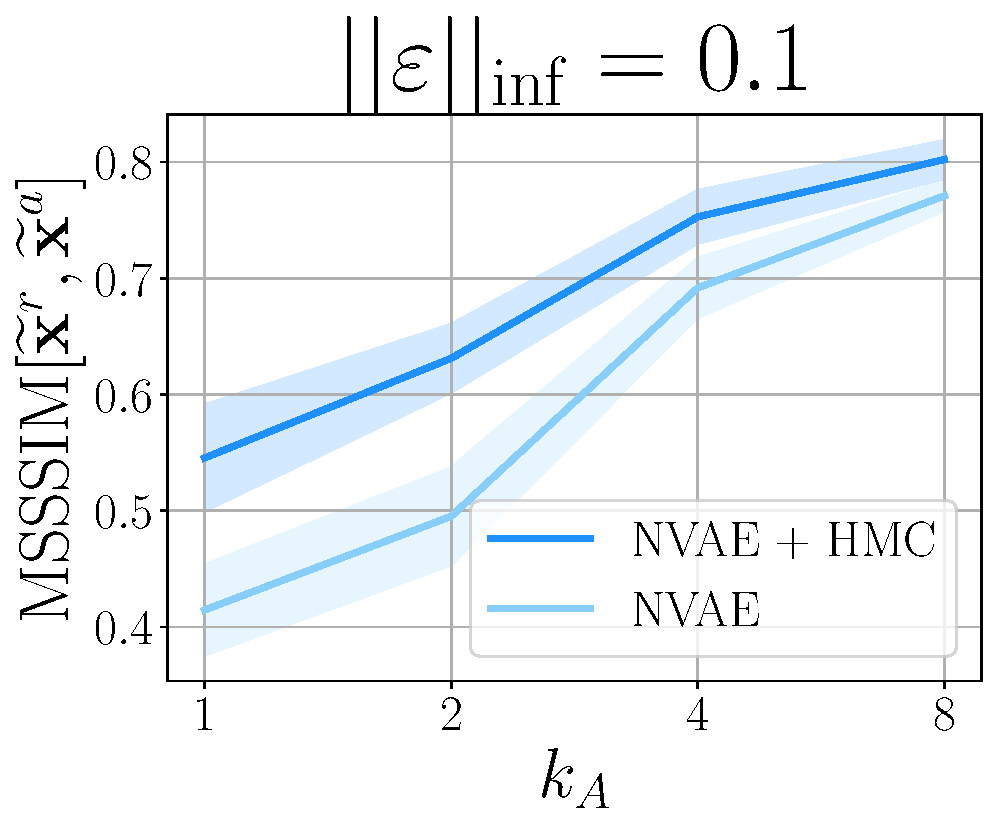
\includegraphics[width=0.4\textwidth]{pics/3_adv_att/nvae_mnist_eps_1.pdf} & 
        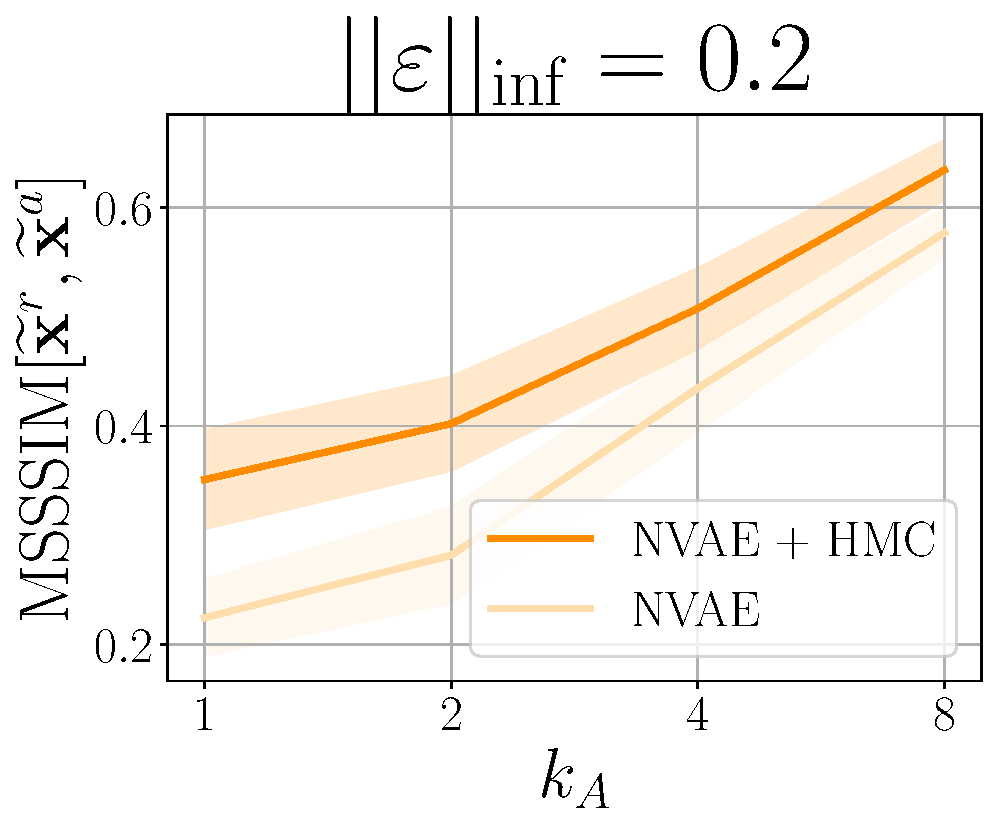
\includegraphics[width=0.4\textwidth]{pics/3_adv_att/nvae_mnist_eps_2.pdf} \\
        \multicolumn{2}{c}{\small (a) The reconstruction similarity for MNIST} \\ \\
        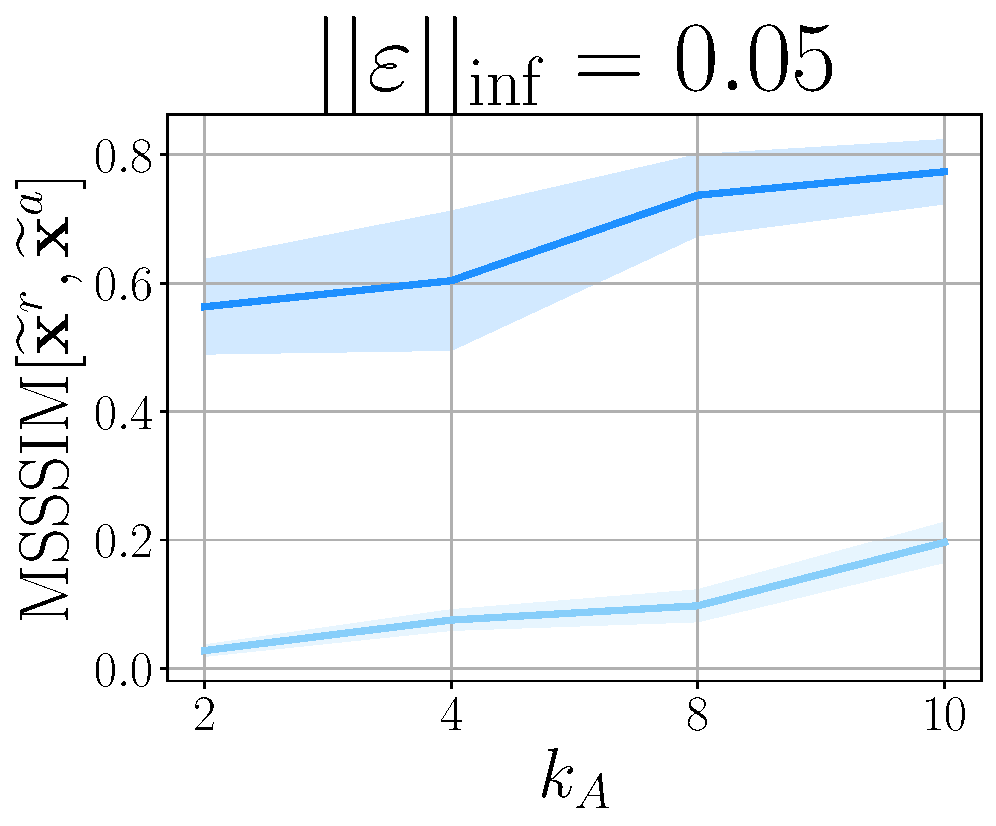
\includegraphics[width=0.4\textwidth]{pics/3_adv_att/nvae_celeba_eps_1.pdf} & 
        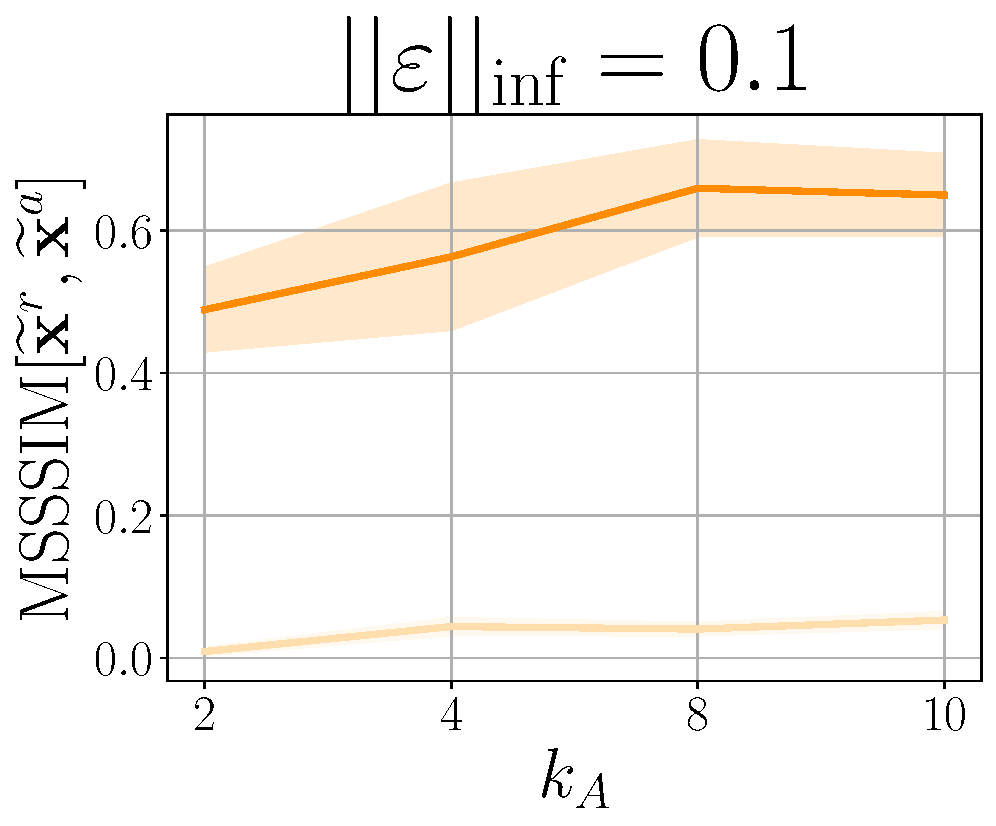
\includegraphics[width=0.4\textwidth]{pics/3_adv_att/nvae_celeba_eps_2.pdf}\\
         \multicolumn{2}{c}{\small (b) The reconstruction similarity for CelebA}\\
    \end{tabular}
    \end{adjustbox}
    \caption[][\baselineskip]{The robustness improvement for the hierarchical model (NVAE) on (a) MNIST and (b) CelebA for two different attack radii. Higher values correspond to more robust representations.}
    \label{fig:nvae_res}
\end{figure}

\subsection{Hierarchical VAE: NVAE}\label{sec:nvae}

\paragraph{Model and datasets} In this section, we explore the robustness of the deep hierarchical VAE (NVAE) \cite{Vahdat2020-xe}, a specific implementation of a hierarchical VAE that works well for high-dimensional data. We attack models trained on MNIST and CelebA \cite{liu2015faceattributes} datasets. We use the weights of the pre-trained model provided in the official NVAE implementation\footnote{The code and model weights were taken from \url{github.com/NVlabs/NVAE}}. 

\paragraph{Attacks construction}
Following \cite{kuzina2021adv} we construct adversarial attacks on the hierarchical VAE by considering higher-level latent variables. That being said, we use latent variables $\{\rvz_{L-k_A}, \rvz_{L-k_A+1}, \dots, \rvz_L\}$ when constructing an attack (\eqref{eq:objective_unsup}). Otherwise, we follow the same procedure we used for VAEs with a single level of latent variables. We assume that the attacker has access to the model's encoder and uses the symmetric KL-divergence as the objective. The radius of an attack is measured with the $L_{\inf}$ norm. For optimization, we use the projected gradient descent with the number of iterations limited to 50 per point. Further details are reported in the Appendix \ref{appendix:vae_attack}.


\paragraph{Results}
In Figure \ref{fig:nvae_res}, we present reconstruction similarity of the reference and adversarial points for both datasets. We observe that the proposed method consistently improves the robustness of the model to the adversarial attack. This result is in line with our theoretical considerations where a flexible class of variational posteriors could help to counteract adversarial attacks and, eventually, deacrease the bias of the class of models measured in terms of the KL-divergence. Additionally, applying the MCMC can further help us to counteract the attack. In Figure \ref{fig:adversarial_examples} (the two bottom rows), we show how an adversarial point (c) is reconstructed without any defence (d) and with the proposed defence (e). In the depicted samples, we have used the top 10 latent variables ($k_A = 10$) to construct the attack with a radius of 0.05. 



% \begin{wrapfigure}{r}{0.62\textwidth}
\begin{figure}[t]
    \centering
    \begin{tabular}{cc}
     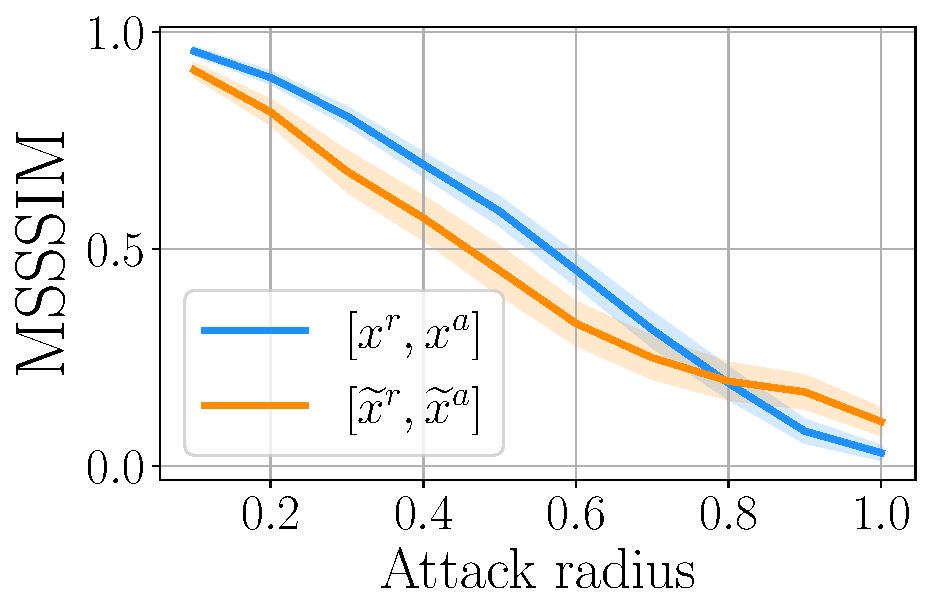
\includegraphics[width=0.4\linewidth]{pics/3_adv_att/attack_mcmc_0_100.pdf} &
     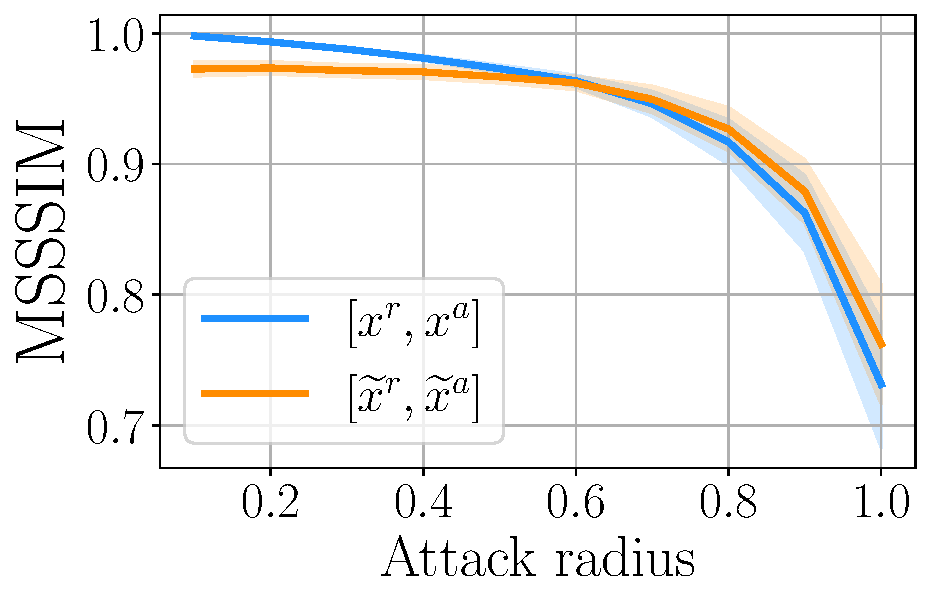
\includegraphics[width=0.4\linewidth]{pics/3_adv_att/attack_mcmc_1_100.pdf} \\
     \multirow{2}{0.45\linewidth}{\centering \small (a) An attacker does not know the defence strategy}&
     \multirow{2}{0.45\linewidth}{\centering \small (b) An attacker knows the defence strategy }\\
     \\
    \end{tabular}
    \caption{Robustness to adversarial attack (with HMC defence). We report similarity of the reference and adversarial point (blue) and their reconstructions (orange).}
    \label{fig:attack_mcmc}
	\vspace*{\baselineskip}
\end{figure}

% \end{wrapfigure}


\subsection{Ablation Study: What if the attacker knows the defence strategy?} \label{sec:ablation}
In our experiments, we rely on the assumption that the attacker does not take into account the defence strategy that we use. We believe that it is reasonable, since the defence requires access to the decoder part of the model, $p_{\theta}(x|z)$, which is not necessarily available to the attacker. 

In this ablation study we verify how the robustness results change if we construct the attack with the access to the defence strategy. We train an adversarial attack with the modified objective \ref{eq:objective_unsup}, which takes into account the HMC step. See Appendix \ref{appendix:attack_mcmc} for more details on the experimental setup. 

In Figure \ref{fig:attack_mcmc} we show the experiment results for various attack radii between 0 and 1. We observe that constructing an attack with such an objective is much harder (Figure \ref{fig:attack_mcmc} (b)).  

% In both cases the reconstructions are almost as close as the initial points, which proves the defence strategy to be successful for this experiment.

% Here we consider the most straightforward approach to construct an attack, which is aligned with the previous works on attacking VAEs. 

% It is, however, possible to use more sophisticated adaptive methods \cite{tramer2020adaptive, athalye2018obfuscated}. We are not aware of the works where such attacks were applied to VAEs and believe that it is an interesting direction for the future work on the topic. 


% \ak{add reference to papers with MCMC defence and attacks, explain that it is out of scope of this paper.}
% In Appendix \ref{appendix:attack_mcmc} we report results of the ablation study, where attacks on the encoder are constructed assuming that the attacker knows the defence strategy and attempts to use it during the attack construction. We observe that using MCMC during the attack construction does not help the attacker. On the contrary, it becomes harder to find a reasonable additive perturbation of the input.

